% Chapter Template

\chapter{Results} % Main chapter title

\label{Chapter3} % Change 3 to a consecutive number; for referencing this chapter elsewhere, use \ref{Chapter3}

\lhead{\emph{Results}} % Change X to a consecutive number; this is for the header on each page - perhaps a shortened title

%----------------------------------------------------------------------------------------
%   SECTION 1
%----------------------------------------------------------------------------------------

\section{Ternary Diagrams}

Using the methods described in Section \ref{Chapter2}, Ternary phase diagrams for each of the four combinations of elements at 298K were produced and reduced - these diagrams are present in \ref{fig:298KTPD}. 

\begin{figure}[ht]
\centering
\begin{subfigure}{70mm}
  \centering
    \includegraphics[width=70mm]{triangleplot_CUZNS298.png}
    \caption{Cu, Zn, S Ternary Diagram}
    \label{fig:CuZnS}
\end{subfigure}%
\begin{subfigure}{70mm}
 \centering
    \includegraphics[width=70mm]{triangleplot_CUZNSN298.png}
    \caption{Cu, Zn, Sn Ternary Diagram}
    \label{fig:CuZnSn}
\end{subfigure}
\begin{subfigure}{70mm}
 \centering
    \includegraphics[width=70mm]{triangleplot_CUSNS298.png}
    \caption{Cu, Sn, S Ternary Diagram}
    \label{fig:CuSnS}
\end{subfigure}
\begin{subfigure}{70mm}
 \centering
    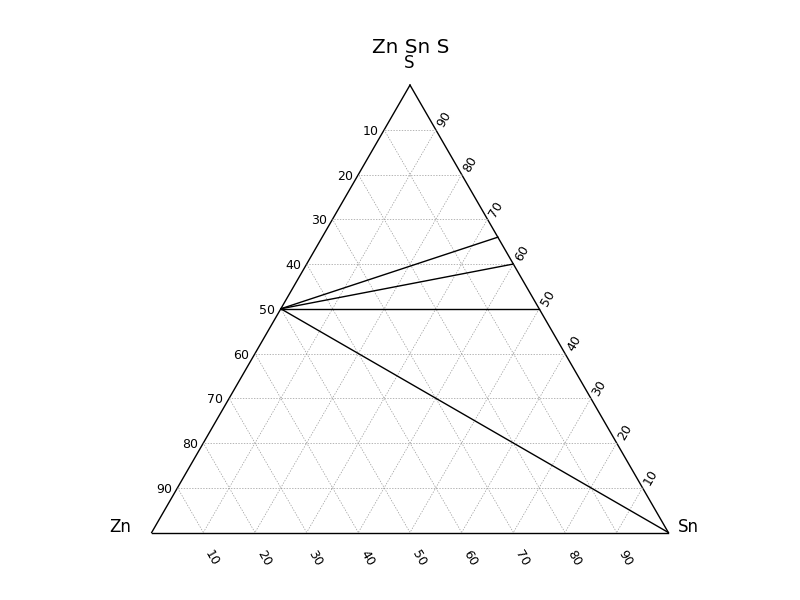
\includegraphics[width=70mm]{triangleplot_ZnSnS298.png}
    \caption{Zn, Sn,S Ternary Diagram}
    \label{fig:ZnSnS}
\end{subfigure}
\caption{Ternary Diagrams of the remaining face, post Tie-line calculations.}
\label{fig:298KTPD}
\end{figure}

%----------------------------------------------------------------------------------------
%   SUBSECTION 1
%----------------------------------------------------------------------------------------

\subsection{Quaternary Diagram}

A quaternary phase diagram was produced by joining the Ternary phase Diagrams along their common edges, and the tie-phases examined. A model of this is presented in \ref{AppendixC}, and a simplified model flattened in the z-axis, with the Cu-Zn-Sn Ternary Phase diagram omitted is presented in \ref{fig:298KQPD}. This diagram effectively presents the sets of tie-lines situated closely to sulphur which join together to form five candidate quasi-ternary phases, whose compositions are as follows: ZnS-SnS-Cu, ZnS-SnS-Cu$_2$S, ZnS-Sn$_2$S$_3$-Cu$_2$S, ZnS-SnS$_2$-Cu$_2$S, ZnS-SnS$_2$-CuS. Each tie-phase was examined to determine whether it held the correct ratio of elements to form CZTS, initially starting with ensuring a 1:1 ratio of Sulphur to the rest of the elements combined. This yielded 2 possible candidates from the group of tie-phases. Subsequently, these two candidates were examined to determine whether they held a composition ratio of 2:1:1 of Cu, Zn and Sn; of the two only one had the correct composition ratio: ZnS-SnS$_2$-Cu$_2$S.


\begin{figure}[ht]
\centering
    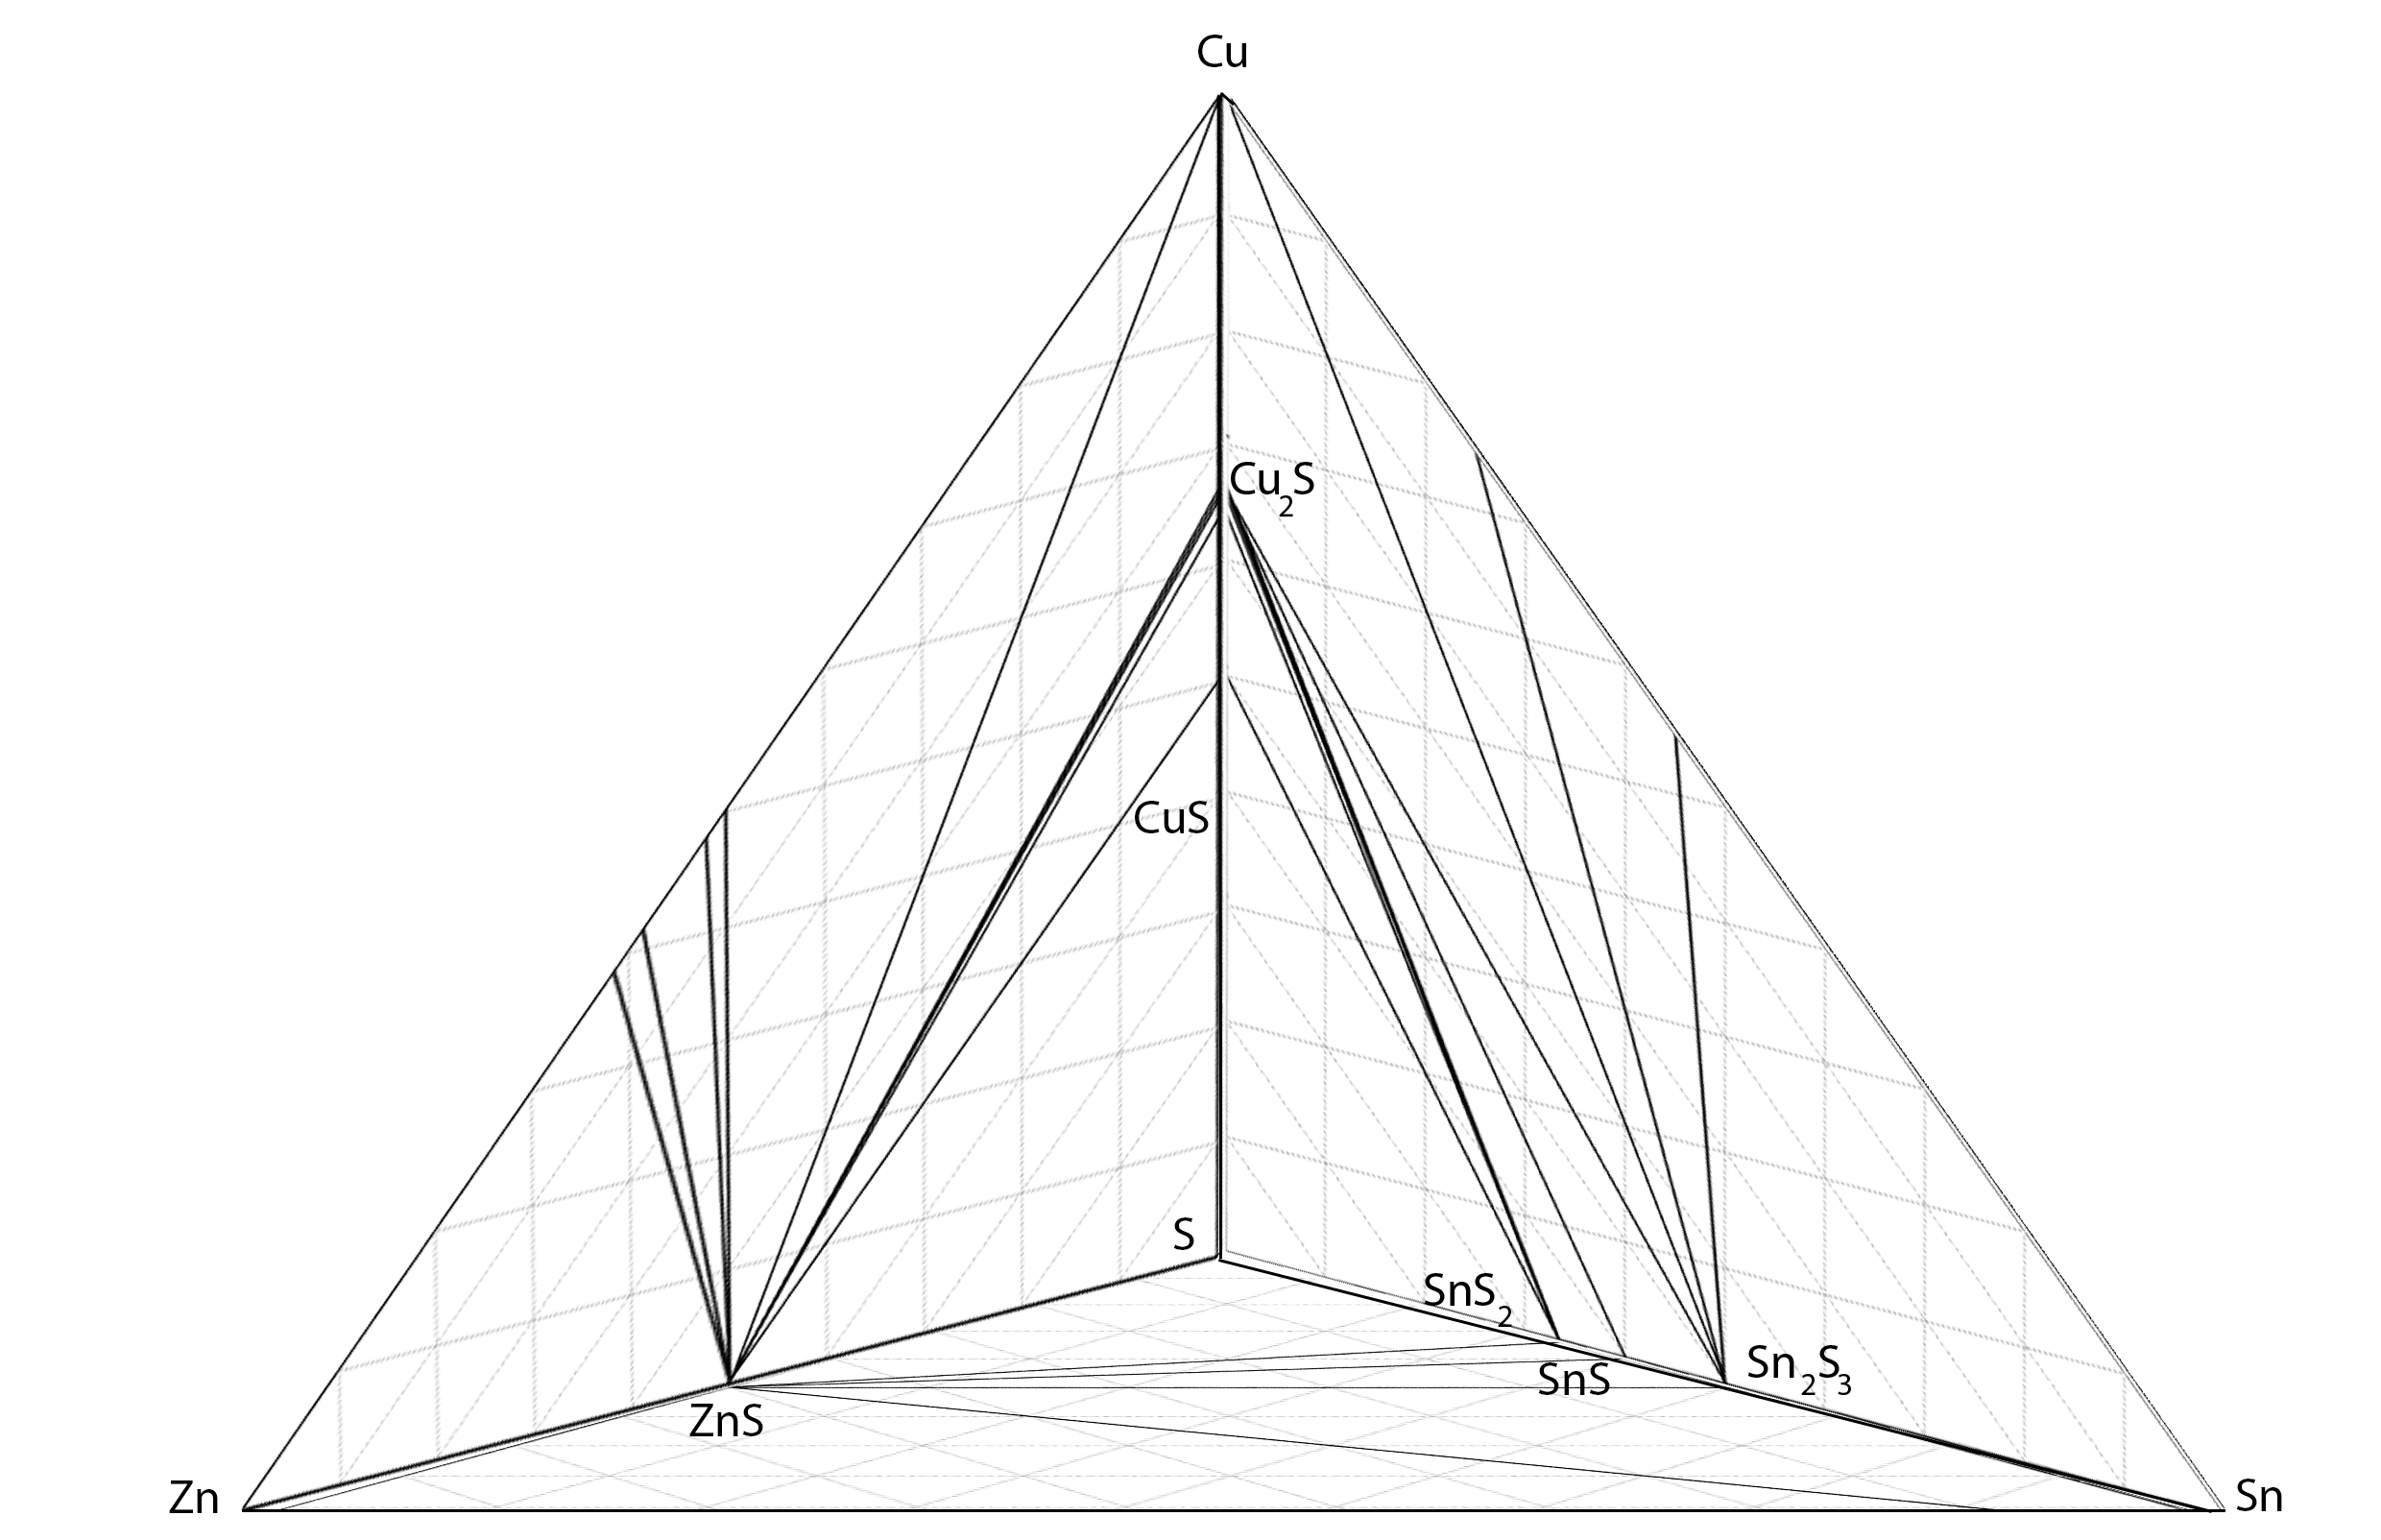
\includegraphics[width=130mm]{FlatQPD.png}
    \caption{Simplified Quaternary Phase Diagram, Omitting the CuZnSn Ternary Phase with the 'corners' of the tie-phases labelled.}
\label{fig:298KQPD}
\end{figure}
%----------------------------------------------------------------------------------------
%   SECTION 2
%----------------------------------------------------------------------------------------

\section{Pseudo-Ternary Diagrams}

Once the ZnS-SnS$_2$-Cu$_2$S pseudo-Ternary system was determined, an initial stoichiometric position for CZTS was determined, presented in \ref{fig:ZnSSn2S3Cu2S}. Alongside the stoichiometric position is labeled distinct compositional phases - areas defined to have a likelihood of containing increased or decreased concentrations of elements. These results fit with those determined by Olekseyuk et al. \citep{Olekseyuk2004}, who performed a more complete analysis of the ZnS-SnS$_2$-Cu$_2$S system at 400$^\circ$C. Their phase diagram has been adapted by Scragg \citep{scragg2011copper} and presented as \ref{fig:Olekseyuk}. Olekseyuk's diagram demonstrates a similar area to find CZTS and includes secondary phases determined through examination of the compound binary phase diagrams for each of the three pairs of compounds: ZnS-SnS$_2$, ZnS-Cu$_2$S and Cu$_2$S-SnS$_2$. Data for these binary phase diagrams at 298K was unavailable, but by examining Olekseyuk's Pseudo-Ternary Phase Diagram it is evident that there are 5 regions where in addition to CZTS there is a single secondary phase, and between these 5 regions exist regions where there are two secondary phases, both secondary phases from the bordering regions are expected to be produced alongside CZTS. As such 6 compositional regions can be designated: Cu "rich", Cu "poor", Zn "rich", Zn "poor", Sn "rich" and Sn "poor". The compositions of these areas are defined in \ref{table:Composition}, as detailed by Scragg \citep{scragg2011copper}.


\begin{table}[h]
\centering
\begin{tabular}{@{}ll@{}}
\toprule
Composition Description & Expected Secondary Phase \\ \midrule
"Cu-poor"               & Cu$_2$ZnSn$_3$S$_8$ + ZnS         \\
"Sn-rich"               & Cu$_2$ZnSn$_3$S$_8$               \\
"Zn-poor"               & CuSnS+Cu$_2$ZnSn$_3$S$_8$/Cu$_2$S    \\
"Cu-rich"               & Cu$_2$S                     \\
"Sn-poor"               & Cu$_2$S, ZnS                \\
"Zn-rich"               & ZnS                      \\ \bottomrule
\end{tabular}
\caption{Difinition of the composition areas in Olekseyuk's Pseudo-Ternary Diagram \citep{Olekseyuk2004}.}
\label{table:Composition}
\end{table}


\begin{figure}
\centering
 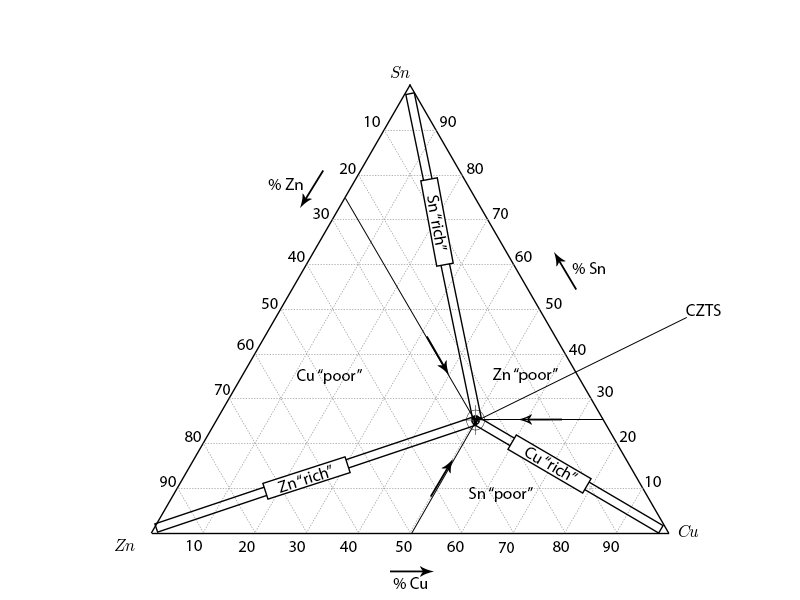
\includegraphics[width=120mm]{ZnSSn2S3Cu2S-general}
    \caption{Stoichiometric location of CZTS, and labeled compositional phases.}
    \label{fig:ZnSSn2S3Cu2S}
\end{figure}
\begin{figure}
\centering
 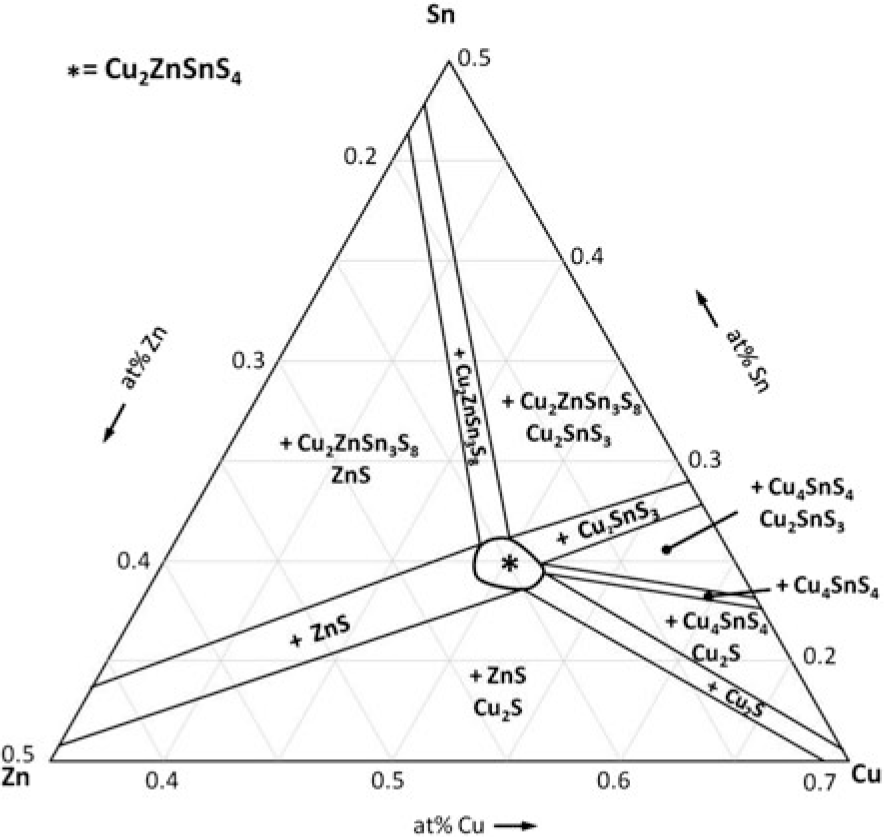
\includegraphics[width=120mm]{OlekseyukTPD}
 \caption{Ternary Phase diagram adapted from Olekseyuk \citep{Olekseyuk2004}, by Scragg \citep{scragg2011copper}. This shows the expected secondary phases at 400$^\circ$C}
    \label{fig:Olekseyuk}
\end{figure}

%----------------------------------------------------------------------------------------
%   SECTION 3
%----------------------------------------------------------------------------------------

\section{Temperature Dependence on the Ternary Phase Diagrams}

In addition to the investigation of the stoichiometric position of CZTS at 298K, the ternary phase diagrams for CZTS were investigated for 600K and 900K. These are presented in 
\ref{fig:600KTPD}, \ref{fig:900KTPD}. These were calculated using the same method as for the 298K Ternary Phase Diagrams, using the data tables in \ref{AppendixA}. As is displayed, there is no variation between the diagrams at 600K and 900K, which is as expected, and the major differences between the 298K and 600/900K Diagrams is the removal and addition of certain phases which were found to be stable at 298K but not at 600/900K, and vice versa. 



\begin{figure}[ht]
\centering
\begin{subfigure}{70mm}
  \centering
    \includegraphics[width=70mm]{triangleplot_CUZNS600-after-full.png}
    \caption{Cu, Zn, S Ternary Diagram}
    \label{fig:CuZnS600K}
\end{subfigure}%
\begin{subfigure}{70mm}
 \centering
    \includegraphics[width=70mm]{triangleplot_CUZNSN600-after.png}
    \caption{Cu, Zn, Sn Ternary Diagram}
    \label{fig:CuZnSn600K}
\end{subfigure}
\begin{subfigure}{70mm}
 \centering
    \includegraphics[width=70mm]{triangleplot_CUSNS600-after.png}
    \caption{Cu, Sn, S Ternary Diagram}
    \label{fig:CuSnS600K}
\end{subfigure}
\begin{subfigure}{70mm}
 \centering
    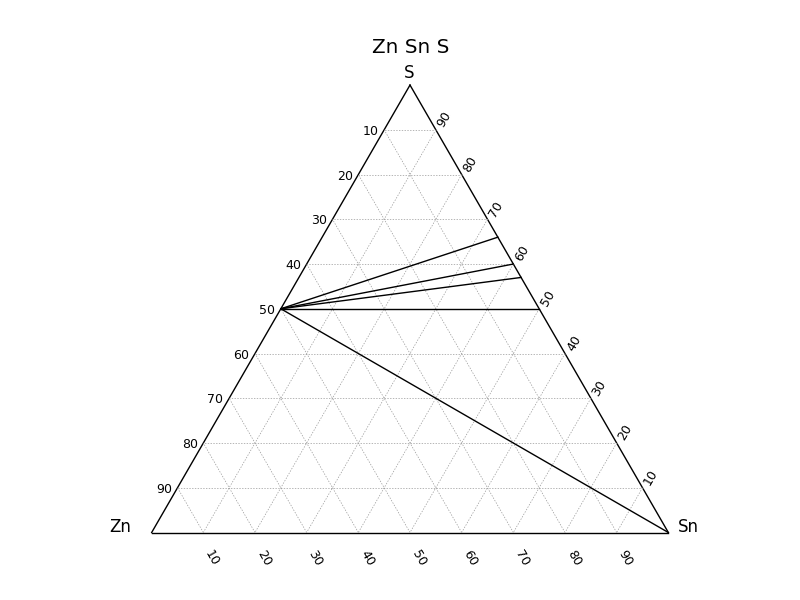
\includegraphics[width=70mm]{triangleplot_ZnSnS600-after.png}
    \caption{Zn, Sn,S Ternary Diagram}
    \label{fig:ZnSnS600K}
\end{subfigure}
\caption{Ternary Diagrams for the CZTS system at 600K}
\label{fig:600KTPD}
\end{figure}


\begin{figure}[ht]
\centering
\begin{subfigure}{70mm}
  \centering
    \includegraphics[width=70mm]{triangleplot_CUZNS600-after-full.png}
    \caption{Cu, Zn, S Ternary Diagram}
    \label{fig:CuZnS900K}
\end{subfigure}%
\begin{subfigure}{70mm}
 \centering
    \includegraphics[width=70mm]{triangleplot_CUZNSN600-after.png}
    \caption{Cu, Zn, Sn Ternary Diagram}
    \label{fig:CuZnSn900K}
\end{subfigure}
\begin{subfigure}{70mm}
 \centering
    \includegraphics[width=70mm]{triangleplot_CUSNS600-after.png}
    \caption{Cu, Sn, S Ternary Diagram}
    \label{fig:CuSnS900K}
\end{subfigure}
\begin{subfigure}{70mm}
 \centering
    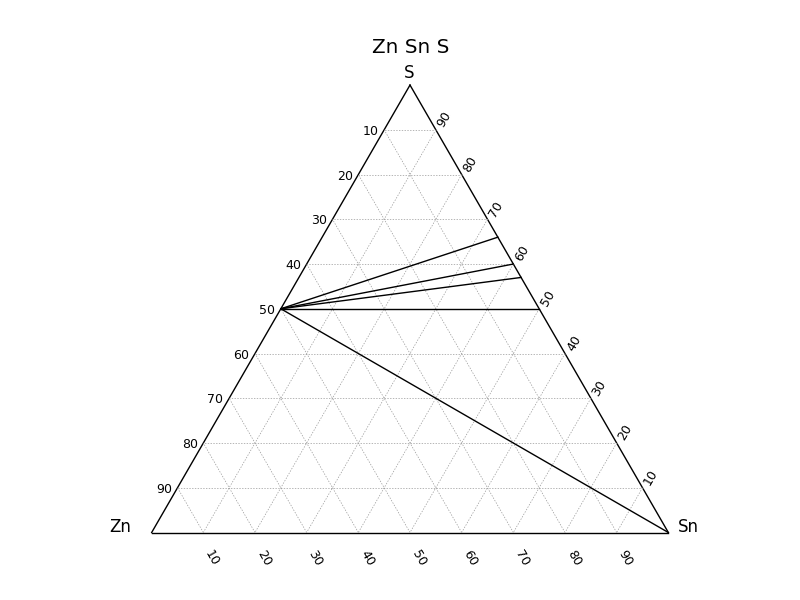
\includegraphics[width=70mm]{triangleplot_ZnSnS600-after.png}
    \caption{Zn, Sn,S Ternary Diagram}
    \label{fig:ZnSnS900K}
\end{subfigure}
\caption{Ternary Diagrams for the CZTS system at 900K.}
\label{fig:900KTPD}
\end{figure}